\section{Chamber Construction}

\subsection{Construction Overview}

\hskip 0.15 in
The chambers were designed with individual holes and holders for
each wire, i.e. a ``strung'' rather than a ``wound'' chamber.  Our 
inspection and assembly procedures were designed to produce devices with 
wires placed and known by external survey to an accuracy of less than 1 mm. 
In addition to accuracy, we have chosen materials and designed 
procedures to insure a quiet and long-lived detector.  The construction 
and wire-stringing techniques were based on our already successful {\tt CLAS} 
drift chamber design.

The three chamber types (called ``regions'', with ``Region1'' abbreviated as 
``R1'', etc.)  share the same basic design elements simply
scaled up in size by a factor of 1.5 for R2 relative to R1 and a factor
of 2 between R3 and R1.  Thus the R3 chambers have a volume which is
about 8 times that of R1 and about 2.5 times that of R2.  
Each chamber is a solid trapezoid in shape, with  
a pair of wire-supporting endplates that bear both the load of the 
wire tensions and the weight of all associated hardware. A representative 
chamber is shown in Fig.~\ref{generic-chamber-sketch}.  The wire tension load in
R1 and R2 was borne by the stiffness of the endplates only, while in
R3 the wire tension was offset 
by compression in a carbon-fiber outer shell and in a set of carbon-fiber 
posts that were part of the chamber construction.  

At the radially outward end of each chamber, a thick ``back-plate'' was 
employed to maintain the relative 
alignment of the endplates, to stiffen the chamber against bending moments, 
and to provide a place to attach gas seals and fittings. At the radially inward 
end of each chamber, the endplates were connected together via a small joining 
piece called the ``nose-plate''.  The hardware fabrication and placement 
was of critical importance to the dimensional accuracy of the chambers.

%%%%%%%%%%%%%%%%%%%%%% Figure : generic chamber sketch %%%%%%%%%%%%%%%%%%%%%%
\begin{figure}[htpb]   
\vspace{4.5cm}
\includegraphics[width=0.5\columnwidth]{generic-chamber-sketch.png}
\caption{\small{Assembly of a typical drift-chamber
(here a R3 sector) highlighting the common components.}}
\label{generic-chamber-sketch}
\end{figure}   
%%%%%%%%%%%%%%%%%%%%%%%%%%%%%%%%%%%%%%%%%%%%%%%%%%%%%%%%%%%%%%%%%%%%%%%%%%

\subsubsection{Endplate and Box Assembly}


The chamber bodies were constructed from the accurately machined plates
(2 endplates, a ``nose plate'' and a ``back plate'').
The endplates themselves were an assembly of a basic plate with precision-drilled
holes to which we bolted and glued stiffener bars.  In the case of
R1 the plate was aluminum and the stiffener bars were stainless steel;
for R2 the plates were G10 and the bars stainless steel and for R3
the plates were an assembly of thin steel plates with a foam interior.

\subsection{Endplate Design and Construction}
\hskip 0.15 in

As noted above our chambers have wires strung from one endplate to 
the other.  Holes are drilled into the endplates into which are
placed feedthrough assemblies meant to hold the wire end.
Each endplate was constructed with 4928 accurately positioned holes into 
which the 
wire-fixture assemblies were placed.  The sense, field, and guard wires in each 
sector were strung between pairs of wire ``feedthroughs''.  As the endplates of 
each chamber faced each other at a 60$^{\circ}$ angle, the wires had to bend 
30$^{\circ}$ at each endplate.  This was accomplished by means of a large radius 
stainless-steel insert at the tip of each feedthrough known as a ``trumpet''.
This trumpet was fitted into an injection-molded Noryl plastic feedthrough.  
All wires were held in place using gold-plated copper crimp pins.  
Low-outgassing epoxy was employed to ensure a gas seal around the feedthroughs 
and crimp pins.  The feedthrough assemblies
are shown in Figs.~\ref{xsect}, \ref{r2_inserts}, and \ref{r3_cut} for R1, R2, 
and R3, respectively.

Fig.~\ref{dc-corner} shows a slice through a chamber endplate (R2 in this case)
showing some of the wire positioning hardware and attachment of the electronics 
boards.
%%%%%%%%%%%%%%%%%%%%%% Figure : DC Sector Schematic %%%%%%%%%%%%%%%%%%%%%%
\begin{figure}[htpb]   
\vspace{4.5cm}Schematic cross-sectional view of the R2 endplate showing
wire-positioning hardware.
\special{psfile=r2_inserts.eps hscale=70 vscale=70 hoffset=-93 voffset=-200}  
\caption{\small{}}
\label{dc-corner}
\end{figure}   
%%%%%%%%%%%%%%%%%%%%%%%%%%%%%%%%%%%%%%%%%%%%%%%%%%%%%%%%%%%%%%%%%%%%%%%%%%



\subsubsection{Inspection and Cleaning}

A visual and tactile inspection was performed on the endplates and 
structural frame upon delivery.  The endplates and structural 
frame underwent a gross cleaning by soaking in a low residue laboratory 
degreasing solution with hand scrubbing, followed by a high-pressure water 
rinse. The parts then received their final cleaning using an ultrasonic 
bath of a laboratory-grade detergent solution.  After two hours they were
removed from the bath and rinsed with de-ionized water and then sprayed 
with methanol to aid drying. Once dry, the parts were heat-sealed in nylon 
bags with a nitrogen atmosphere to await assembly.

Smaller parts such as feedthroughs and hardware were cleaned using a 
bench-top ultrasonic cleaner with laboratory detergent, followed by a 
de-ionized water rinse and a dousing of methanol to facilitate drying.  
In addition, the injection-molded parts are specified to be free of silicon 
mold releases.



\subsection{Wire Choice}
\hskip 0.15in

Our ``thin endplate'' design required minimizing wire tensions and
thus diameter or the wire.  The real key to reducing wire tension is to
make the field wires (which are much larger than the sense wires) as 
thin as possible and to make them out of low-density metal.  In this 
section we describe our choices for sense, field and guard wires.
We had to trade off the robustness and more uniform drift velocity
afforded by large diameter sense wire with the disadvantages that they
required higher electric fields, a potential problem for our high-density
signal amplifier boards.

In general, designers have chose very small diameter sense wires because they
require lower operating voltates.
The sense wire for all of our chambers, supplied by the Luma
Sweden Company, consists of 30-$\mu$m diameter gold-plated tungsten.  
The previous CLAS drift chambers used 20-$\mu$m diameter wire for the
sense wires.  We decided to use the thicker 30-$\mu$m wire for two 
reasons: first, it is significantly tougher making it easier to handle without
accidental kinking and less likely to break, and second, to operate at the same 
gas gain as chambers with the thinner wire requires a high voltage setting 
(approximately 300 V higher) and this results in a higher field throughout the cell
and a more linear drift velocity function.  As will be discussed later,
we determined that our on-chamber high-voltage distribution boards could
handle the higher operating voltages.

Tungsten was chosen because of its durability, 
and the gold-plating of the wires, amounting to a thickness of 0.127~$\mu$m, 
ensures chemical inertness as well as a smooth surface finish.  The expected 
electronics gain and thresholds dictated that the gas gain be a few times 
10$^4$.  Under this condition, the electric field at the surface of the sense 
wires is $\approx$200~kV/cm.  The field-wire diameter was chosen to ensure 
that the electric field at their surface remained below 50~kV/cm to minimize 
conditions which could cause unwanted cathode emissions.  We note that
our choice violated the ``20~kV/cm rule'' proposed by Fabio Sauli and others
to reduce cathode emission.  Our own studies showed that there was no cathode
emission below 50~kV/cm from any wire with good surface finish.  Each batch
of wire was tested with our test device (ref:patent) to ensure that at operating field 
values there was no emission.  

We chose 80-$\mu$m gold-plated Cu-Be wire for our field wire.
It is very tough, and is easily plated and resists ``flaking'' of the gold
plating.  The 80-$\mu$m diameter choice was made to obtain the minimum
radius that would satisfy our surface electric field limit.  This small
diameter is important because it means that the field wires could be strung 
at lower tension than a more dense wire, with minimal gravitational sag.  
This minimizes the forces on the endplates which we wanted to keep as 
thin as possible to maximize the solid-angle of the sensitive area of
the chambers.


\subsection{Construction Materials}

\hskip 0.15 in
Due to the complex geometry of CLAS and the difficulty of removing and repairing 
drift chambers, it was crucial to minimize chamber aging.  Care was taken to 
ensure that all materials in contact with the gas volume were clean and ``chamber 
safe'' as defined in Ref~\cite{kadyk}.  All construction was carried out in 
Class-10000 or better clean rooms.

The drift-chamber frames were made primarily of aluminum (R1), fiberglass (R2),
or steel-clad structural foam (R3).  The aluminum and steel endplates were 
manufactured with machine oils and were subsequently cleaned with  
Micro-laboratory detergent from the Cole-Parmer Instrument Company.  The 
fiberglass endplates were machined without any lubricating oils.  Immediately 
prior to chamber assembly all endplates were sequentially cleaned with 
detergent,
 deionized water, and alcohol, and then blown dry with pure nitrogen gas.  The 
wire feedthroughs, trumpets, and crimp pins were cleaned in an ultrasonic bath 
with detergent and then rinsed in a second ultrasonic bath with deionized water.

During construction three different types of epoxy were used in areas exposed 
to the chamber gas.  Shell Epon resin 826 mixed with Versamid 140, and 
Scotchweld varieties 210 and 2216 were employed.  These mixtures have been 
studied extensively and found not to outgas significantly~\cite{nasa}.

The on-chamber gas tubing employed is mainly stainless steel, with some
nylon tubing included for gas manifolds.  Special care was taken during
all steps of construction and testing to ensure that no oils or
silicones contacted any of the chamber materials.

\subsection{Chamber Wire Stringing}

\hskip 0.15 in

Because all of the chambers have the same shape, differing only in
size and some materials, we strung them all using the same basic method.
They were gravity-strung using the same basic methodology 
used when stringing the previous {\tt CLAS} drift chambers.  The detector box 
assembly was mounted to a stringing fixture.  The frame was connected to 
the fixture using attachments that allow the chambers to rotate along 
the center of mass.  This permitted safe and easy 
rotation of the detector by hand.  A gantry crane was used to lift the 
detector onto and off the stringing fixture and to raise the small end of 
the detector to account for the stereo angles.

The stringing fixture was very basic.  It was mounted to the floor using 
concrete anchors.  This minimizes floor obstruction as the box must be 
rotated to the opposite side to string the second set of wires.  The box 
and frame assembly were placed far enough away from the uprights such that 
they did not interfere with stringing activities.  There was a gross 
adjustment using 
the gantry crane to lift the telescoping side and pin it on the adjustment 
collar.  The collar had a fine adjustment to allow setting it at the most 
favorable stringing angle.  The detector box was rotated 180$^\circ$ to 
string the second superlayer.

Once the detector was installed onto the fixture, wire feedthrough 
insulators were inserted and glued into each hole. Special care was 
taken to use only the minimal amount of glue required to provide a solid gas 
seal and to prevent glue contamination inside the detector.  Once one 
endplate was filled, the assembly was rotated such that the other side 
could be done.  Once all wire feedthrough inserts were in place, the box 
was pre-tensioned.

With nearly 130,000 wires to be threaded through the chambers and only 2 years 
for construction, it was important to minimize the time required to string 
each wire.  All chambers were strung with 
the wires running vertically.  The stringing technique involved attaching a 
small steel needle to the wire before threading it through the feedthrough in 
the upper endplate.  The wire was then despooled and gravity acted to bring the 
wire close to the feedthrough in the lower endplate.  A small magnet was then 
used to pull the needle and wire through the lower feedthrough.  After the upper 
crimp pin was attached and remaining slack in the wire was removed, the lower 
crimp pin was slid over the wire and stringing weights were attached to set the 
proper tension.  The lower crimp pin was then attached, completing the process.
  
Wires that wrapped around each other while being threaded through the chamber 
were a major contribution to stringing inefficiency. To avoid the wrapping
problem, a machine was built to spool the wire through the chambers at a fast 
and smooth rate.  Another important development was the design of a crimp pin 
that accepted both the tungsten and copper-beryllium wire types.  Using a 
thick-walled 
copper pin ensured a good crimp through a range of gap settings~\cite{sbc}.  This 
eliminated the need to use separate crimping tools, each requiring frequent 
calibrations.  This was possible because the wire position was determined by the 
radius of the trumpet at the end of the feedthrough inside of the chamber, and 
not by the concentricity of the pin, feedthrough, and endplate-hole diameters. 
As a result, the average time to string a wire was less than 4 minutes.

\subsection{Region One Construction (Special Considerations)}

The R1 chambers were designed and constructed through a collaboration 
of Idaho State University and Jefferson Laboratory.  These 
chambers are located about 2~m from the target, 
before particles enter the magnetic field of the torus,
and are thus key to good angular resolution. 

As is seen from the generic assembly sketch of a chamber (see Fig.~\ref{chambers-and-torus}),
the R1 chambers have a similar shape to the R2 and R3 chambers, differing in
scale and in some material choices.
Most notably, the endplates are constructed of aluminum with stainless
steel stiffener bars.

The main challenges in the R1 construction and design came about because
of the small wire spacing (8~mm between the sense and field wires).  This
increased the electrostatic attraction of neighboring wires if they were
not perfectly and symmetrically placed, and it also made the physical act
of stringing the wires more difficult.

Wires with opposite voltage are electrostatically attracted.  If perfectly
placed in a symmetric array the forces would cancel each other. 
However, the sense wires might be slightly misplaced and so they would feel
a force which, if the tension were below a critical value, would increase
and pull them further out, further increasing the force, and so on until 
the wire begins to oscillate and then spark.  For our electric field configuration
this critical tension was about 3~g, substantially below our nominal
tension of 20~g.



\subsection{Region Two Construction (Special Considerations)}

\hskip 0.15 in 
The R2 chambers, which were designed and constructed by Old Dominion University 
in collaboration with Jefferson Laboratory, are the middle of the three  
drift-chamber packages.  They track all charged particles in the magnetic field 
of the torus near the point of maximum sagitta.  The six identical R2 sectors 
are approximately equilateral triangular boxes with 3 m sides. 
They are located at a radius of $\approx$3~m from the nominal target location.  
  
The R2 chambers were designed with ultra-thin endplates which were thin enough
to be wholly within the ``shadow'' cast by the torus cryostat; in other words,
the full length of the wires is in the active fiducial volume of CLAS12. 
All chamber support hardware and electronics had to fit 
entirely within this shadow region.


Fig.~\ref{dc-corner} shows a slice through a chamber endplate (R2 in this case)
showing some of the wire positioning hardware and attachment of the electronics 
boards.
%%%%%%%%%%%%%%%%%%%%%% Figure : DC Sector Schematic %%%%%%%%%%%%%%%%%%%%%%
\begin{figure}[htpb]   
\vspace{8cm}Schematic cross-sectional view of the R2 endplate showing
wire-positioning hardware.
\special{psfile=img/r2_inserts.eps hscale=70 vscale=70 hoffset=0 voffset=50}  
\caption{\small{}}
\label{dc-corner}
\end{figure}   
%%%%%%%%%%%%%%%%%%%%%%%%%%%%%%%%%%%%%%%%%%%%%%%%%%%%%%%%%%%%%%%%%%%%%%%%%%


The R2 chambers have to operate 
in a magnetic field up to 2~T, and the chambers have to withstand any rapid 
changes in magnetic field, such as what might occur due to a magnet quench.
The R2 endplates are constructed from 2-cm thick Stesalit 4411W, a disordered 
epoxy-fiberglass composite commonly used in wire-chamber construction
\cite{stesalit}, and known not to cause aging problems~\cite{stesalitaging}.  
Using a nonconducting material eliminates any possible forces on the endplate 
due to eddy currents produced during a magnetic-field quench.  

The ``stesalit'' composite is not very stiff and, if not reinforced, would
bend excessively under the load of wire tension.  So, as in the case of
the R1 chambers, the R2 endplates were a composite structure with
stainless steel stifferners.  Fig.~\ref{dcr2-endplate} shows an assembly drawing of an R2 endplate.

%%%%%%%%%%%%%%%%%%%%%% Figure : generic chamber sketch %%%%%%%%%%%%%%%%%%%%%%
\begin{figure}[htpb]   
\vspace{10cm}
\begin{picture}(35,35)
\put(10,-10)
{\hbox{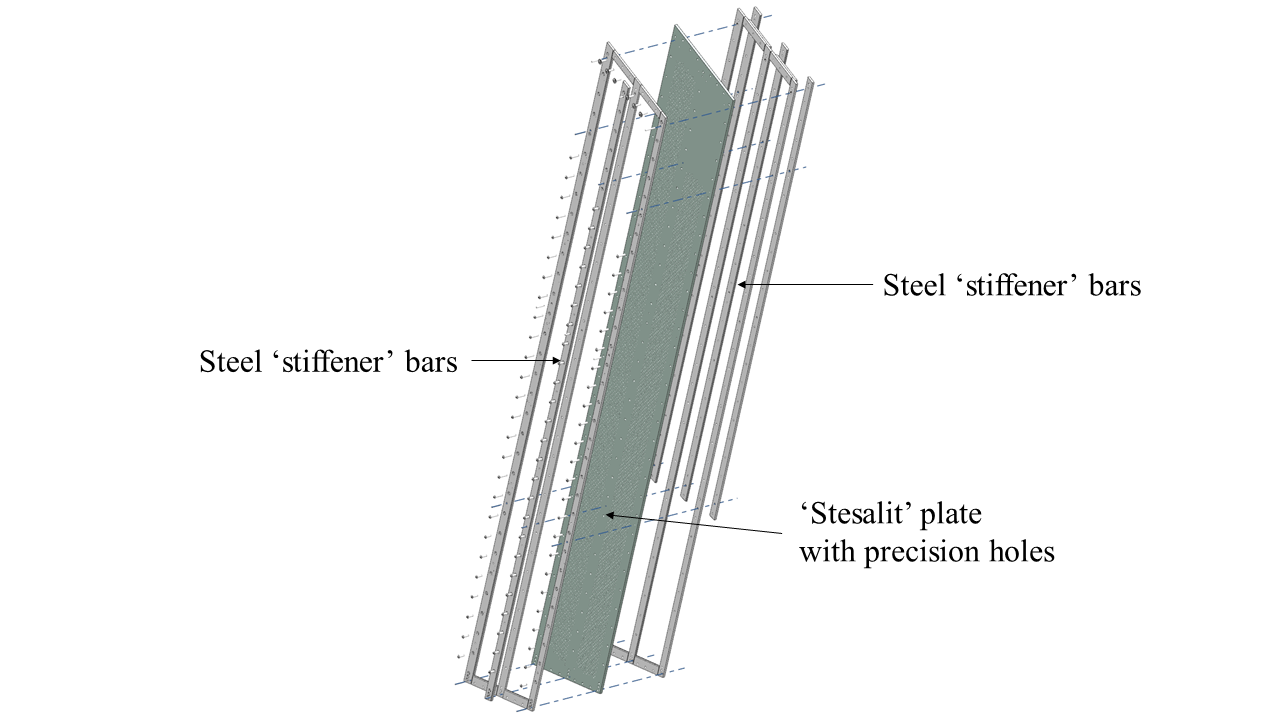
\includegraphics[width=0.5\columnwidth,natwidth=610,natheight=642]{img/dcr2-endplate.png}}}
\end{picture}
\caption{\small{A R2 endplate assembly.}}
\label{dcr2-endplate}
\end{figure}   
%%%%%%%%%%%%%%%%%%%%%%%%%%%%%%%%%%%%%%%%%%%%%%%%%%%%%%%%%%%%%%%%%%%%%%%%%%

It also allows 
the trumpets that position the wires to be essentially flush with the endplates, 
rather than having to insulate the trumpets from the conducting endplates as in 
the other two Regions (see Fig.~\ref{dc-corner}).  This reduced the thickness of 
the inactive region by 1 to 2~cm.




 



\subsection{Region Three Construction}

\hskip 0.15 in
The R3 chambers were designed and constructed at Jefferson Laboratory.  
They had the same general shape as the other chambers but were larger,
4 m on a side so the wires were as long as 4 m.
To reduce the gravitational sag of these very long wires we
strung them at 40 grams, twice the nominal tension of 20 grams.

%%%%%%%%%%%%%%%%%%% Figure : Region Three Cross Section %%%%%%%%%%%%%%%%%%
\begin{figure}[htpb]
\vspace{7.9cm}
\caption{\small{Assembly drawing of a R3 chambers showing the component
parts and highlighting the Carbon fiber tubes at the entrance face and
the carbon-foam composite plate at the exit, which supported the endplates
agains the wire tension.}}
\label{r3_cut}
\end{figure}
%%%%%%%%%%%%%%%%%%%%%%%%%%%%%%%%%%%%%%%%%%%%%%%%%%%%%%%%%%%%%%%%%%%%%%%%%%%

Because these are the final tracking chambers, multiple scattering
at the chamber entrance is not as important as multiple scattering that
occurs at a R1 or a R2 chamber, for example.  This allowed us to 
build a chamber in which the endplates were not supported only on
their ends.  At the entrance face we included 7 thin-walled Carbon
fiber tubes to span the gap and hold the endplates apart.  At the
exit face the endplates were coupled to a triangular carbon-foam-carbon
composite plate which similarly supported the wire tension.







